\documentclass{article}
\usepackage{textcomp}
\usepackage{graphicx} 
\usepackage[margin=1in]{geometry}
\usepackage{amsmath}
\usepackage{booktabs}
\usepackage{subcaption}
\usepackage{float}
\usepackage{chemfig}
\usepackage[version=4]{mhchem}
\setchemfig{bond offset=2pt, atom sep=2.3em}
\usepackage{mathtools}
\usepackage{xcolor}
\usepackage{wrapfig}


% setting up shiz for citations. use \autocite{} 
\usepackage[
  colorlinks=true,
  linkcolor=blue!80!black,
  citecolor=blue!80!black,
  urlcolor=blue!80!black
]{hyperref}
\usepackage[style=chem-acs, autocite=inline]{biblatex}
\DeclareFieldFormat{labelnumber}{\textit{#1}}
\makeatletter
\renewcommand{\bibleftbracket}{(}
\renewcommand{\bibrightbracket}{)}
\makeatother
\addbibresource{references.bib}
\ExecuteBibliographyOptions{doi=true}
\usepackage{cleveref}


%%%%%%%%%% clever setup
% Fully spelled out, lowercase
\crefname{figure}{figure}{figures}
\crefname{table}{table}{tables}
\crefname{section}{section}{sections}
\crefname{equation}{equation}{equations}

% No parentheses for equations
\creflabelformat{equation}{#2#1#3}

% Uniform style
\crefformat{figure}{#2Figure~#1#3}
\crefformat{table}{#2Table~#1#3}
\crefformat{section}{#2Section~#1#3}
\crefformat{equation}{#2Equation~#1#3}

\Crefformat{figure}{#2Figure~#1#3}
\Crefformat{table}{#2Table~#1#3}
\Crefformat{section}{#2Section~#1#3}
\Crefformat{equation}{#2Equation~#1#3}
%%%%%%%%%%


% changing TOC to have smaller "contents" word
\usepackage{tocloft}
\renewcommand{\cfttoctitlefont}{\Large\bfseries}
\renewcommand{\cftaftertoctitle}{\hfill}

\usepackage{listings}

\lstset{
    language=Python,
    basicstyle=\ttfamily\small,
    keywordstyle=\color{blue},
    stringstyle=\color{green!60!black},
    commentstyle=\color{gray},
    showstringspaces=false,
    frame=single,
    breaklines=true
}

\usepackage{caption} \captionsetup{justification=raggedright,singlelinecheck=false} \setlength{\captionmargin}{0pt}

\usepackage{etoolbox}

\pretocmd{\appendix}{
  \crefname{section}{appendix}{appendices}
  \crefname{subsection}{appendix}{appendices}
  \crefname{subsubsection}{appendix}{appendices}

  \Crefname{section}{Appendix}{Appendices}
  \Crefname{subsection}{Appendix}{Appendices}
  \Crefname{subsubsection}{Appendix}{Appendices}
}{}{}

% Define a real "appendix" type
\crefname{appendix}{appendix}{appendices}
\Crefname{appendix}{Appendix}{Appendices}
\crefformat{appendix}{#2Appendix~#1#3}
\Crefformat{appendix}{#2Appendix~#1#3}


\title{Determination of Kinetic Parameters and Applications of Measured Rate Law for Iodination of Acetone}
\author{Ethan Bowen, Ryan Lange, Megan Lynch, Kyle Wodehouse}
\date{April 2026}

\begin{document}
%% TITLE PAGE SETUP !!!

\begin{titlepage} 
\centering
\vspace*{2cm}
{\Huge \textbf{Determination of Kinetic Parameters and Applications of Measured Rate Law for Iodination of Acetone} \par}
\vspace{1.5cm}
{\Large Ethan Bowen \\ Ryan Lange \\ Megan Lynch \\ Kyle Wodehouse \par}
\vspace{0.5cm}
{\large  \textit{``Capybaras''} \par}
\vspace{1.5cm}
{\large University of Delaware \\ Chemical \& Biomolecular Engineering \par}
\vspace{0.5cm}
{\large Prof. Dongxia Liu \par}
\vspace{0.5cm}
{\large April 2026 \par}
\vfill
\end{titlepage}
\begin{abstract}
Accurate parameterization of reaction rate laws is essential for reactor design,  process optimization, and scale-up in chemical engineering applications. The  acid-catalyzed iodination of acetone was studied to determine its rate law and temperature dependence using the method of initial rates. Reaction orders were determined using linear, multiple linear, and nonlinear regression. Nonlinear regression yielded the most precise parameter estimates, with 95\% confidence intervals of $\alpha = 1.026 \pm 0.063$, $\beta = 0.954 \pm 0.068$, and $\gamma = -0.134 \pm 0.67$ for acetone, hydrochloric acid (HCl), and iodine, respectively, consistent with a pseudo-equilibrium mechanism. The activation energy and pre-exponential factor were determined from a linearized Arrhenius plot to be $E_a = (114.4 \pm 5.6)$ kJ/mol and $\ln(A) = (36.0 \pm 2.2)$ (standard error). The measured activation energy is in statistical agreement with the literature consensus of approximately 86--89 kJ/mol. However, this agreement is tenuous given that only three temperature points were used, producing a critical t-value of ~12.7 and a confidence interval wide enough to encompass nearly any physically reasonable activation energy.  The experimentally determined rate law was applied to numerically model autocatalytic behavior in a BSTR and to size a CSTR for iodoacetone production at 353 K and 80\% acetone conversion, yielding a nominal volume of 274 L. A Monte Carlo simulation ($N = 100{,}000$) produced a 90\% confidence interval of 58--1,290 L, with uncertainty dominated by the Arrhenius parameters $E_a$ and $\ln(A)$. Additional rate measurements across a wider temperature range between 303--353 K are recommended to most efficiently constrain reactor volume uncertainty along with having more statistical power compare the apparent activation energy to literature values.
\vspace{1em}

A practical survey of pneumatic pressure measurement instruments was conducted to understand their functional roles in process systems. Instruments examined included Bourdon gauges, pressure transducers, mass flow controllers, and control valves. Operation of a pneumatic pressure rack enabled direct observation of pressure regulation, signal transmission, and feedback control behavior. Differences between mechanical and electronic measurement devices were evaluated in terms of response time, sensitivity, and stability. Control valve performance under varying setpoints illustrated the importance of proper controller tuning in maintaining steady-state operation. This exercise provided practical insight into the integration of instrumentation and control hardware and emphasized their role in ensuring safe, stable, and efficient industrial processes.


\end{abstract}


\tableofcontents

\section{Introduction}

The ability to quantify reaction kinetics is central to the design and scale-up of chemical reactors. Errors in rate parameters propagate directly into vessel sizing, residence time, and ultimately process economics. Additionally, catalysis is central to the chemical industry, as over 90\% \autocite{armor_new_1991} of industrial chemical processes rely on catalysts to achieve economically viable reaction rates and selectivities \autocite{ertl_handbook_2008, rothenberg_catalysis_2008, armor_history_2011, liu_catalytic_2011, yang_selective_2025, paunovic_exploring_2026, li_critical_2025, xin_roadmap_2026}.  This report documents two laboratory exercises that explore each discipline through hands-on experimentation. The first study examines the acid-catalyzed iodination of acetone to determine its rate law and temperature dependency. The second exercise provides a practical overview of a pneumatic pressure rack, focusing on the hardware used to monitor and control fluid pressure in industrial settings.

The iodination of acetone is a standard model reaction for kinetic studies because the reaction progress is easily visible. As iodine is consumed, its characteristic red-brown color fades, allowing the reaction rate to be monitored using UV-visible spectrophotometry. The goal of this experiment was to determine the reaction orders for acetone, hydrochloric acid (HCl), and iodine using the method of initial rates. By measuring rate constants at varying temperatures, the activation energy ($E_a$) and pre-exponential factor ($A$) were calculated from the Arrhenius equation \autocite{arrhenius}. These parameters are essential for engineering applications, as they allow for the accurate sizing of industrial reactors, such as continuous stirred-tank reactors (CSTRs), and the modeling of complex behaviors like autocatalysis in batch stirred-tank reactors (BSTRs).


\subsection{Objectives}
The primary objective of the kinetics lab was to determine the rate law and Arrhenius parameters for the acid-catalyzed iodination of acetone through the method of initial rates. Using the experimentally determined rate law, a CSTR was sized for a specified production target and a Monte Carlo simulation was performed to quantify uncertainty in the volume prediction. Additionally, a BSTR with autocatalytic behavior was numerically modeled. 

\section{Iodination of Acetone}
\subsection{Background \& Theory}
\subsubsection{Reaction Rate Orders}

The iodination of acetone is commonly used in undergraduate laboratories to demonstrate chemical kinetics as the reaction rate is easily monitored by the red-brown iodine color disappearing, which demonstrates the decrease in the concentration of iodine as the reaction progresses \autocite{birk_three_1992}. The reaction proceeds through three elementary steps where the second step is the rate limiting step.

% \begin{figure}[H]
%     \centering
%     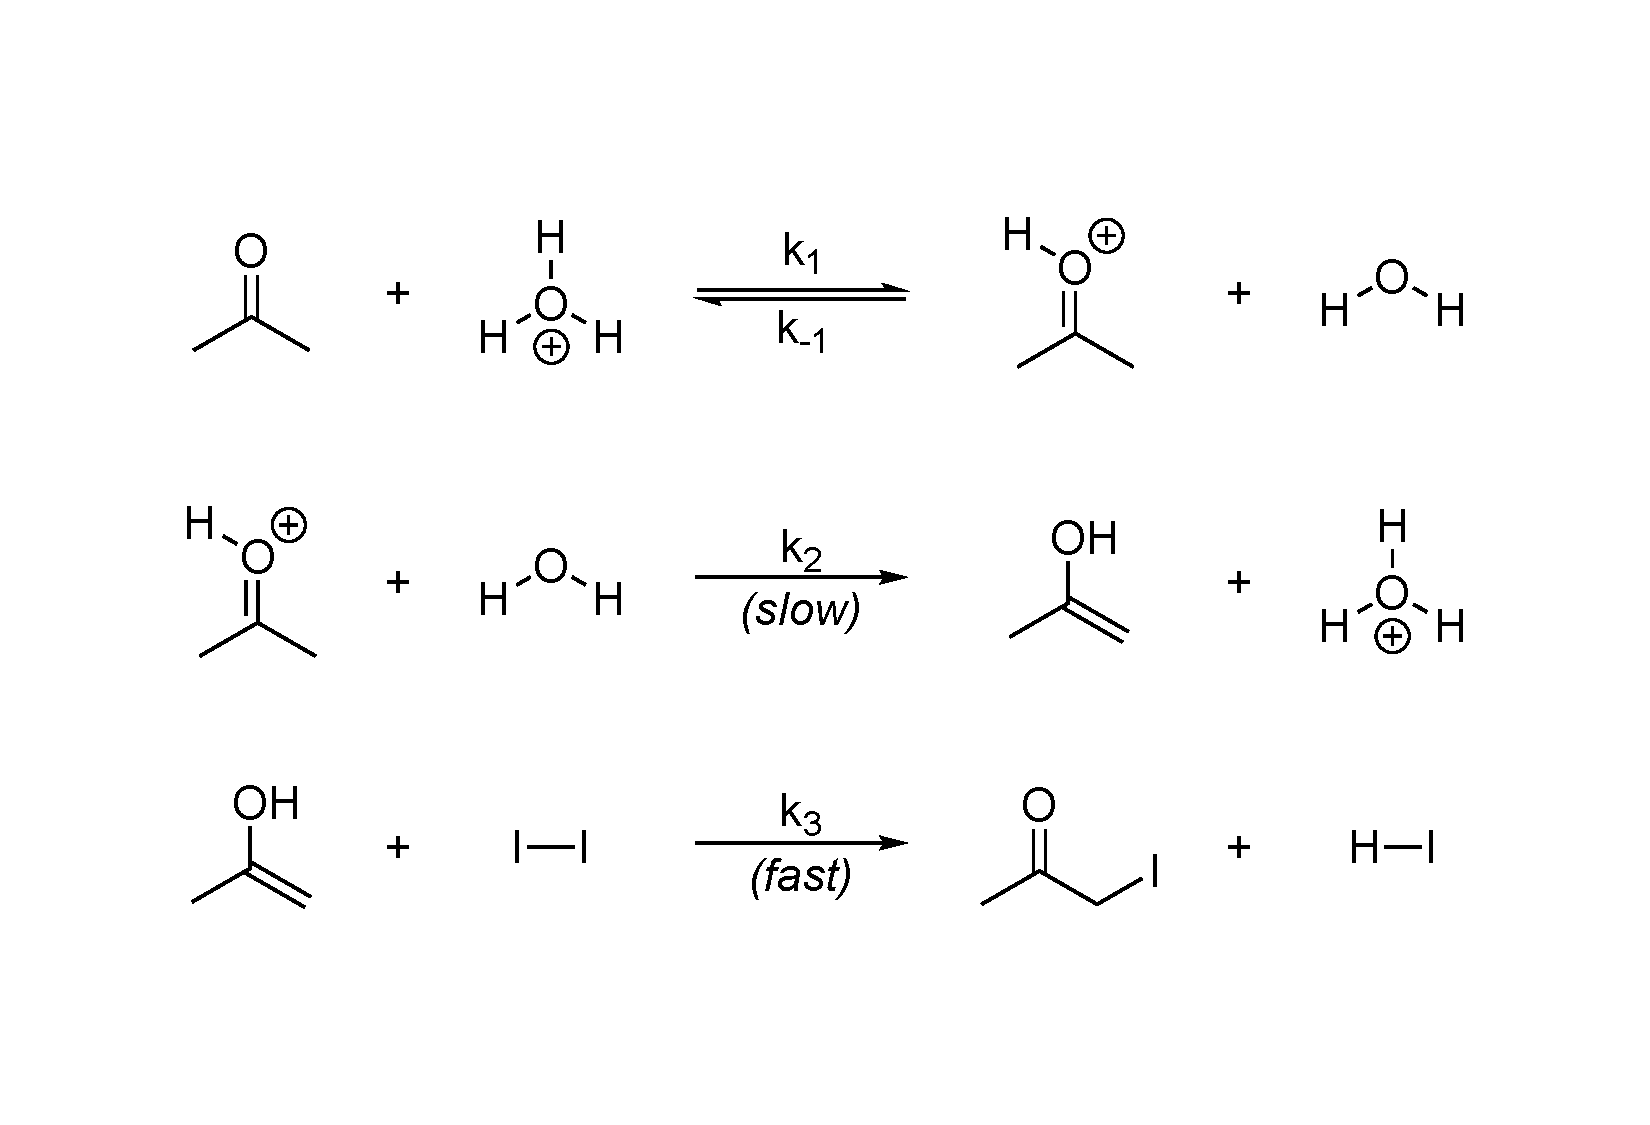
\includegraphics[width=0.95\linewidth]{figures/chemdraw.pdf}
% \end{figure}

\begin{align}
    % Step 1: Protonation equilibrium
    \chemfig{CH_3-C(=[2]O)-CH_3} \quad + \quad \ce{H3O+} \quad
    &\xrightleftharpoons[k_{-1}]{\quad k_1 \quad} \quad
    \chemfig{CH_3-[0]C(=[2]OH^{+})-[0]CH_3} \quad + \quad \ce{H2O}
    \\[1em]
    % Step 2: Enol formation (slow, rate-determining)
    \chemfig{CH_3-[0]C(=[2]OH^{+})-[0]CH_3} \quad + \quad \ce{H2O} \quad
    &\xrightarrow{\quad k_2 \quad} \quad
    \chemfig{CH_2=[0]C(-[2]OH)-[0]CH_3} \quad + \quad \ce{H3O+}
    \\[1em]
    % Step 3: Iodination (fast)
    \chemfig{CH_2=[0]C(-[2]OH)-[0]CH_3} \quad + \quad \ce{I2} \quad
    &\xrightarrow{\quad k_3 \quad} \quad
    \chemfig{CH_3-[0]C(=[2]O)-[0]CH_2I} \quad + \quad \ce{HI} \label{mechanism}
\end{align}
\setcounter{equation}{0}
\vspace{1em}


The rate law may be derived by applying the pseudo-equilibrium approximation to the fast pre-equilibrium step  \autocite{dongxia} and the result is shared in \cref{theoRate} where $k_\textbf{obs}$ is the experimentally measurable reaction rate constant. The concentration of acetone is noted as $[\mathrm{Ac}]$ to condense the following equations.

\begin{equation}
    \mathrm{Rate}_2 = \frac{k_2 k_1}{k_{-1}} [\mathrm{Ac}][\mathrm{H_3O^+}] = k_\mathrm{obs} [\mathrm{Ac}][\mathrm{H_3O^+}] \label{theoRate}
\end{equation}

The method of initial rates is a common way to determine the form of the rate law. In this method the reaction rate is measured near the start of the reaction where the changes in reactant concentrations are negligible \autocite{initialrates}. 
\begin{equation}
    \mathrm{Rate} = k [\mathrm{Ac}]^{\alpha} [\mathrm{H_3O^+}]^{\beta} [\mathrm{I_2}]^{\gamma} \label{powerlaw}
\end{equation}

To find the reaction order with respect to HCl, iodine, and acetone concentration the reaction rate was measured while changing the concentration of the component of interest and holding the other concentrations constant. The rate equation may be linearized by taking its logarithm (\cref{linearized_rate}).
\begin{equation}
\ln(\mathrm{Rate}) = \ln (k) + \alpha \ln ( [\mathrm{Ac}] ) + \beta \ln ([\mathrm{H_3O^+}]) + \gamma \ln ([\mathrm{I_2}])  \label{linearized_rate}
\end{equation}


From \cref{linearized_rate} it is seen that when holding the rate constant $k$ and all other initial concentrations fixed the apparent orders may be measured as the slope of a best fit line. This relationship is presented mathematically in \cref{alpha}. The other orders, $\beta$ and $\gamma$, can be measured similarly to $\alpha$ by varying the initial concentrations of HCl or iodine.

\begin{equation}
    \alpha = \frac{\partial (\ln \mathrm{Rate})}{\partial (\ln [\mathrm{Ac}])} \label{alpha}
\end{equation}


\subsubsection{Activation Energy Determination}
The Arrhenius equation relates the reaction rate constant to the reaction's activation energy and the reaction temperature \autocite{arrhenius}. The equation may be linearized by taking its logarithm, and the linearized form of the equation is useful to find the activation energy, $E_a$, and pre-exponential factor, $A$, from linear regression (\cref{eq:arrhenius_for_EaA}).

\begin{equation}
    k = A \exp \left( \frac{- E_a}{RT}\right) \quad \longrightarrow  \quad \underbrace{\ln (k)}_y = \underbrace{\ln (A)}_b + \underbrace{\frac{1}{T}}_x \underbrace{\left(\frac{-E_a}{R} \right)}_m \label{eq:arrhenius_for_EaA}
\end{equation}

\subsubsection{Beer-Lambert Law}

The Beer-Lambert law \autocite{swinehart_beerlambert_1962} relates the absorption of light to the properties of the material through which the light is traveling. It states that the intensity of transmitted light decreases exponentially with the concentration of the absorbing species and the path length of the medium:

\begin{equation}
A = \epsilon b c
\end{equation}

where $A$ is the absorbance, $\epsilon$ is the molar absorptivity, $b$ is the path length, and $c$ is the concentration. This law is fundamental in spectrophotometric analysis and allows us to determine the concentration of $\mathrm{I_2}$ in the reaction mixture by measuring its absorbance. Absorbance measurements may be converted to concentration measurements with a linear calibration curve provided by course organizers (\cref{eq:calibrationcurve}). 

\begin{equation}
    A = m [I_2] + b \quad \longrightarrow \quad [I_2] = \frac{A-b}{m} \label{eq:calibrationcurve}
\end{equation}
\noindent
The $m$ and $b$ parameters for each spectrophotometer are included in \cref{app:signals}. 

\subsection{Methods}

\subsubsection{Safety}

Lab coats, nitrile gloves, and splash goggles were worn to prevent contact with chemicals and to avoid being pricked by any needles. HCl, iodine, and acetone were handled in the fume hood, where the sash was kept under the designated line. Chemicals were properly disposed of into the liquid waste containers, blunt-tip needles were disposed into the sharps container, and gloves were disposed of into the solid waste container. A safety shower and eye wash station were present if needed. Detailed SDS information for each reagent is included in \cref{app:SDS}.

\subsubsection{Procedure}
The recirculating water bath was turned on and set to the desired reaction temperature prior to beginning the experiment. The reactor was charged with deionized water and acetone by transferring the liquids with a graduated cylinder. The graduated cylinders were weighed before and after each addition to determine the mass of liquid added. The reactor agitator and peristaltic sipper pump were then turned on and the stirring speed was recorded from the digital display. Syringes with blunt-tip needles were labeled for iodine and HCl and filled accordingly. 

HCl was injected into the reactor through the top port, and iodine was injected after the reactor temperature stabilized and UV–visible spectrophotometer data collection was started. Each syringe was weighed before and after injection into the reactor to determine the mass of reagent delivered. Absorbance data was collected for approximately 100 seconds before stopping data collection, turning off the sipper pump, and draining the reactor. The reactor was rinsed two times with 650 mL of deionized water before the next reaction.


\subsubsection{Standard Run}
The reagent concentrations and masses for a ``standard'' run are included in \cref{tab:standardrun}. Volume targets were used to approximately dose reagents into syringes/graduated cylinders while recorded masses before and after addition to the reactor were used to calculate concentrations for each reaction. For reactions where the concentration of one reagent was varied, the target mass of water was adjusted to maintain a target total volume of 650 mL.

\begin{table}[H]
    \centering
    \caption{Reagent concentrations for a standard acetone iodination reaction run.}
    \label{tab:standardrun}
    \begin{tabular}{lcccc}
        \toprule
        Reagent & Desired Conc. (M) & Stock Conc. (M) & Volume (mL) & Mass (g) \\
        \midrule
        HCl      & 0.02  & 1.00  & 13.00    & 13.00     \\
        Iodine   & 0.002 & 0.10  & 13.00    & 13.00     \\
        Acetone  & 2.00     & 13.60 & 95.59 & 75.51  \\
        Water    & 45.13 & 55.52 & 528.41 & 528.41 \\
        \midrule
        Total & & & 650.0 & 629.9 \\
        \bottomrule
    \end{tabular}
\end{table}


\subsubsection{Apparatus}
\cref{fig:reactordiagram} shares a diagram of the reactor setup used. The reactor is a jacketed glass 800 mL reactor. The heating jacket water was heated to a temperature set at 30, 35, or 40 ºC, but the temperatures used in calculations were thermocouple readings which were slightly lower.

\begin{figure}[H]
    \centering
    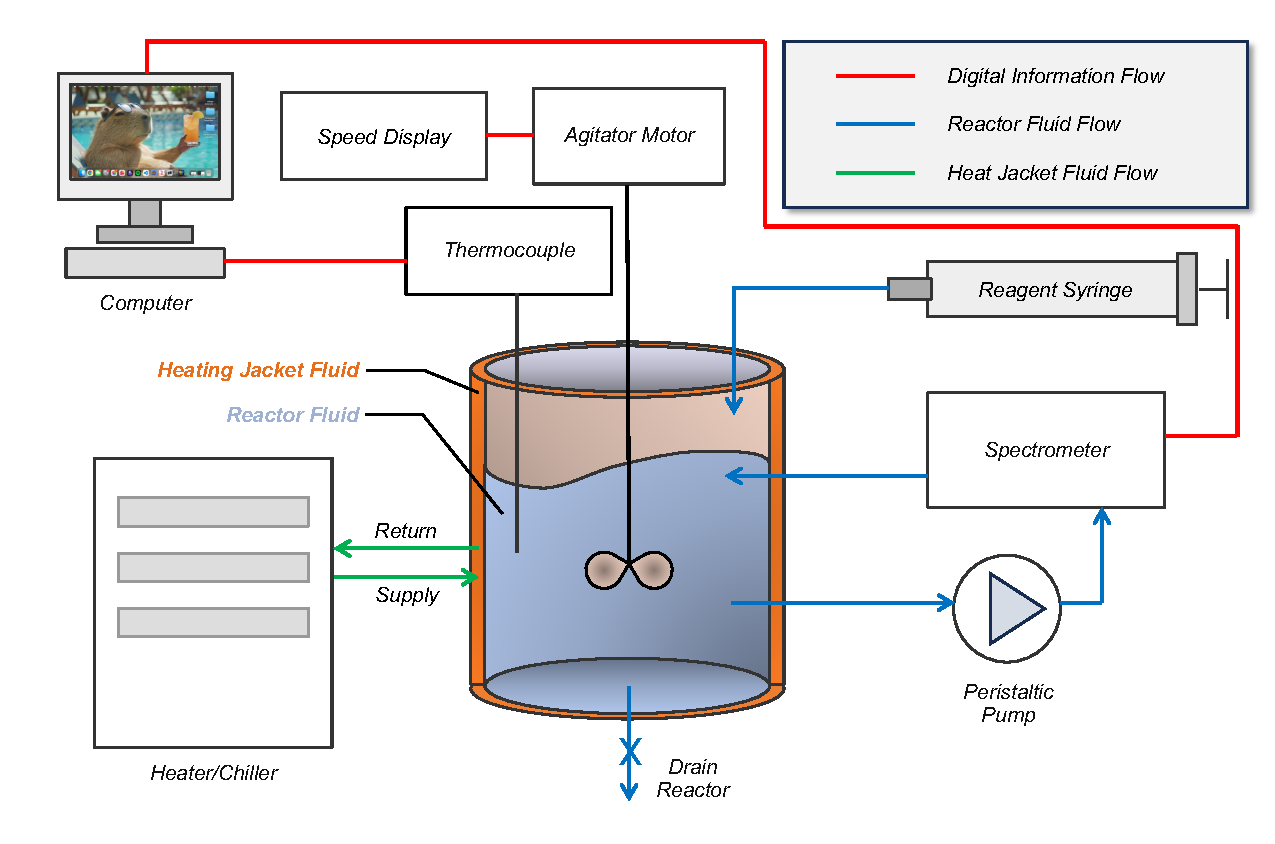
\includegraphics[width=\linewidth]{figures/reactor_diagram.pdf}
    \caption{Diagram of reactor apparatus.}
    \label{fig:reactordiagram}
\end{figure}

\subsubsection{Temperature Measurements}
The temperature inside the reactor was measured with a thermocouple at a sampling rate of 1 measurement per second. The start time of each reaction was recorded to compute the average and standard deviation of the temperature readings during the time absorbance measurements were recorded.

\subsubsection{UV-visible Spectroscopy Measurements}
Absorbance measurements at 510 nm were recorded with an Ocean Optics spectrophotometer using the Vernier Logger Pro software at a sampling rate of 1 measurement per second.  Outliers were removed by random sample consensus  \autocite{RANSAC} (see \cref{app:processing} for more detail). 

\subsection{Results and Discussion}
\subsubsection{Observed Reaction Orders}

A power-law rate law relationship in the form of \cref{powerlaw} was investigated. \Cref{fig:reactionOrders} shares the collected reaction rate data linearized and fit with linear regression. From \cref{fig:reactionOrders}, the 95\% confidence interval on the acetone order is (0.96 $\pm$ 0.61), for HCl it is (0.98 $\pm$ 0.43), and the reaction order with respect to iodine is (-0.2 $\pm$ 1.8). These confidence intervals were computed as the standard error in the slope multiplied by the critical t-value at 95\% confidence with 1 degree of freedom.

\begin{figure}
    \centering
    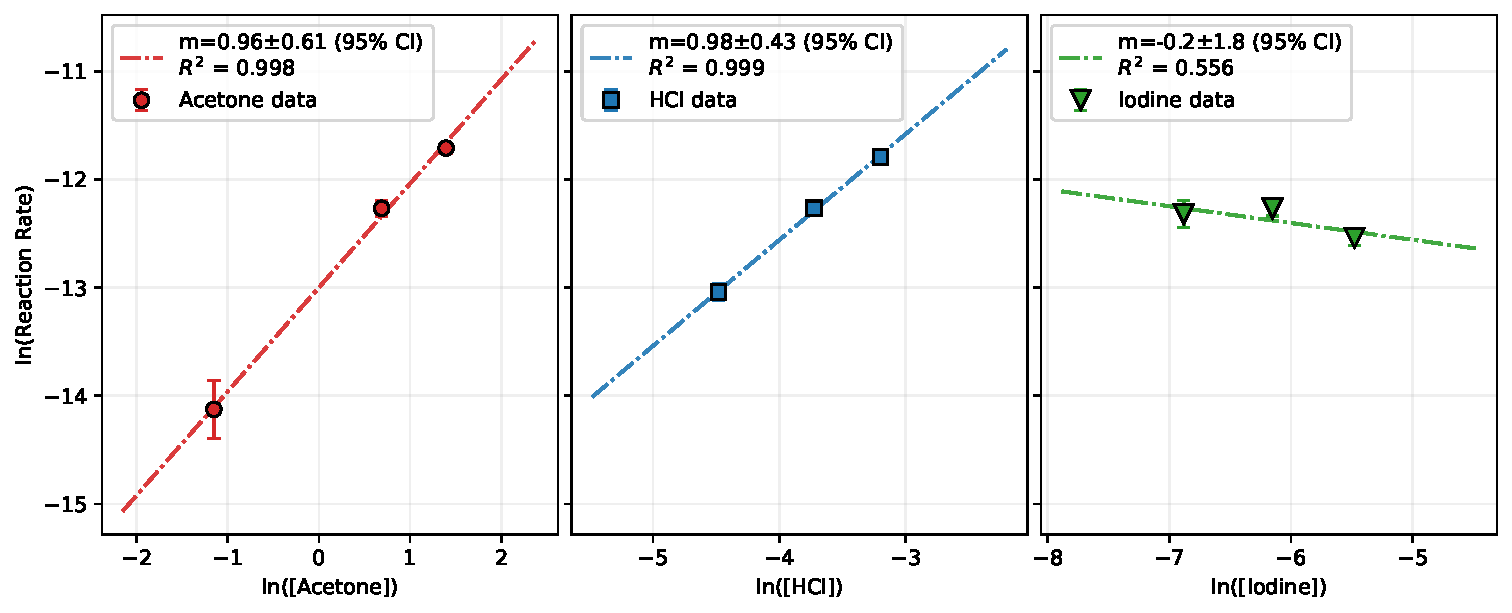
\includegraphics[width=\linewidth]{figures/orderplot.pdf}
    \caption{Reaction orders from the slope of a linearized form of the rate equation. Each subplot shares the same y-axis. Plotted error bars are asymmetric and were propagated from the error in the measured reaction rate in accordance with Hites  \autocite{hites_calculating_2017}. The slope of the linear fit lines correspond to the observed reaction order in accordance with \cref{alpha}. Though it appears like many of the points have no error bars, they are simply smaller than the size of the plotted marker.}
    \label{fig:reactionOrders}
\end{figure}

It is shown in \cref{fig:reactionOrders} that the observed reaction orders are in statistical agreement with the theoretical ($p_\alpha=0.559, p_\beta = 0.648, p_\gamma = 0.464$). Details of statistical tests are shared in \cref{app:tests}. The high $R^2$ values for the HCl and acetone experiments shows a strong agreement between a linear fit and the collected data, consistent with a power law rate law. The large relative error and poor $R^2$ value for the set of experiments seeking to determine the reaction order with respect to iodine are consistent with the zeroth order derived from first principles \autocite{dongxia}. The data plotted in \cref{fig:reactionOrders} are tabulated in \cref{app:orderData}. 



\subsubsection{Multiple Linear and Nonlinear Regression}
A source of systematic error in the linear regression analysis to determine the reaction order with respect to each component was the slightly different concentrations from run to run. Additionally, the confidence intervals provided by linear regression of two parameters using three data points are large as the t-statistic only has one degree of freedom. There are two approaches to fitting rate data to a rate law which accounts for the slight variations in initial concentrations of the other reagents: multiple linear regression and nonlinear regression. 

The reaction order data was collected at the same temperature such that the rate constant, k, was held constant. This allows for fitting the rate equation data to a linear equation of the form shared in \cref{multiplelinear} where $\beta_0=\ln(k)$ and $\beta_i$ is the observed reaction order for species i.

\begin{equation}
    \hat{y} = \beta_0 + \sum_{i=1}^{n} \beta_i [X]_i \label{multiplelinear}
\end{equation}

Nonlinear regression fits the measured reaction rate directly to the proposed power law form of the rate equation without requiring linearization. Unlike linear regression, there is no closed-form solution to nonlinear regression, so the Levenberg-Marquardt algorithm  \autocite{levenberg_method_1944, marquardt} was used to minimize the sum of the squared residuals across the collected data. Importantly, the residuals minimized by nonlinear regression differ from those minimized by multiple linear regression, since linearization applies a nonlinear transformation to the residuals. This accounts for the small discrepancy in fitted parameters between the two methods. The results from each regression method are shared in \cref{tab:regressionResults}.



\begin{table}[H]
    \caption{Reaction orders using different regression methods. Indicated errors are 95\% confidence intervals where the degrees of freedom is the number of data points minus the number of model parameters.}
    \centering
    % \vspace{0.5em}

    % {\large
    % $\mathrm{Rate} = k [\mathrm{Acetone}]^{\alpha}
    % [\mathrm{H_3O^+}]^{\beta}
    % [\mathrm{I_2}]^{\gamma}$
    % }
    % \vspace{0.5em}
    \begin{tabular}{c|cccc}
    \toprule
    Method & $\alpha$ (Acetone) & $\beta$ (HCl) & $\gamma$ (Iodine) & $\ln(k)$ \\
    \midrule
    linear regression & $0.98 \pm 0.43$ & $0.96 \pm 0.61$ & $-0.2 \pm 1.8$ & --- \\
    multiple linear regression & $0.97 \pm 0.11$ & $1.092 \pm 0.068$ & $-0.14 \pm 0.10$ & $-10.27 \pm 0.80$ \\
    nonlinear regression  \autocite{marquardt} & $1.026 \pm 0.063$ & $0.954 \pm 0.068$ & $-0.134 \pm 0.067$ & $-10.26 \pm 0.15$ \\
    \bottomrule
    \end{tabular}
    \label{tab:regressionResults}
\end{table}

The reaction orders from linear regression shared in \cref{tab:regressionResults} are in statistical agreement with the orders predicted from the pseudo-equilibrium and rate limiting step approximations. Another way to arrive at this conclusion is that the theoretical values (1st order in HCl and acetone and 0th order in iodine) are included within the 95\% confidence intervals. The confidence intervals for nonlinear and multiple linear regression are smaller as there are more degrees of freedom ($\nu = \ $\# data points $-$ \# model parameters $=3$). Observed orders from nonlinear regression for  acetone and HCl are also in agreement with the theoretical orders ($p_\alpha = 0.273, p_\beta = 0.117$), but the order for iodine is not in agreement ($ p_\gamma = 0.008$). 

Despite this  disagreement, $\gamma = -0.134$ was retained in subsequent calculations rather than setting it to zero, as the value is small in magnitude and its physical effect on the computed rate is negligible at the concentrations studied. The sensitivity analysis in \cref{sec:cstr} confirms this, showing  uncertainty in $\gamma$ contributes less than 6\% relative uncertainty to the predicted reactor volume, compared to roughly 70\% from the Arrhenius parameters. The statistical disagreement is therefore acknowledged but does not materially affect the engineering conclusions drawn from the rate law.


\subsubsection{Activation Energy}
\label{sec:EA}

Rate constants were calculated following the determination of reaction orders using the method of initial rates, where reactant concentrations undergo negligible change over the first 5–10\% of the reaction. The rate equation was rearranged to solve for the rate constant (\cref{rateconstant}), where $\alpha$ and $\beta$ are the reaction orders obtained from nonlinear regression.

\begin{equation}
    k = \frac{\mathrm{Rate}}{\mathrm{[Acetone]_0^\alpha [HCl]_0^\beta [I_2]_0^\gamma}} \label{rateconstant}
\end{equation}

The error of the natural log of the rate constant is readily calculated from the linearized form of the rate equation. The details of this derivation along with an example calculation are shared in \cref{app:errorProp}, but the result is presented in \cref{errorbars_lnk}.

% remember to put information in the derivation about how the error in the concentrations is way negelible compared to the fit params

\begin{equation}
\delta \ln(k) = \sqrt{
    \left(\frac{\delta \mathrm{Rate}}{\mathrm{Rate}}\right)^2
    + \ln([\mathrm{Ac}])^2 \, \delta\alpha^2
    + \ln([\mathrm{H_3O^+}])^2 \, \delta\beta^2
    + \ln([\mathrm{I_2}])^2 \, \delta\gamma^2}
\label{errorbars_lnk}
\end{equation}

\Cref{fig:activation_energy} shares a linearized Arrhenius plot for the activation energy measurement experiments and was generated with rate constants computed with \cref{rateconstant} and the average temperature measurement during the time absorbance measurements were collected.

\begin{figure}[h]
    \centering
    
\includegraphics[width=0.9\linewidth]{figures/activationenergy.pdf}
    \caption{Determination of activation energy (Ea) from linearized form of the Arrhenius equation. Rate constants were calculated from the method of initial rates (\cref{rateconstant}), 
    and the error bars were computed from \cref{errorbars_lnk}. Details for computing the 95\% confidence interval are shared in \cref{app:plotCI}.}
    \label{fig:activation_energy}
\end{figure}

The high $R^2$ value between the collected data and the linear fit along with a visibly linear relationship indicates a strong linear relationship, consistent with the Arrhenius equation. The error bars on the collected values for ln(k) are symmetric, though it should be noted that the error bars of the logarithm being symmetric indicate the error bars for the rate constant, $k$, itself will be asymmetric. The error bars in the logarithm of $k$ are smaller than the 95\% confidence interval in the linear regression which is consistent with a central assumption in ordinary least squares that uncertainty is primarily in the response variable rather than the predictor.


The experimentally determined activation energy is ($114.4 \, \pm \, 5.6)$ kJ mol$^{-1}$ (standard error), and the pre-exponential factor itself is large and would have an associated asymmetric error, so instead its natural log is reported. The determined value of $\ln(A)$ is ($36.0 \pm 2.2$) (standard error). These results are in statistical agreement ($p = 0.126$) with Albery's value for acetone iodination \autocite{albery_measurement_1969} of ($86.6 \pm 0.23$) kJ mol$^{-1}$. Interestingly, Delluva  \autocite{delluva2015} mistakenly claims that Albery's \autocite{albery_measurement_1969} measurements were for the bromination of acetone while in reality they were for the iodination of acetone. A summary of literature results for acetone iodination are shared in \cref{tab:literatureEA} which is largely adapted from Table 7 in Albery \autocite{albery_measurement_1969}. 

\begin{table}[h]
\centering
\caption{Energies of activation for the iodination of acetone. Reported energies were converted to kJ mol$^{-1}$ and reported errors are standard errors.}
\begin{tabular}{lc}
\toprule
Source & $E_a$ (kJ mol$^{-1}$) \\
\midrule
Rice and Kilpatrick  \autocite{rice_measurement_1923} & $86.62 \pm 0.25$ \\
Bell and Bamford (in Albery  \autocite{albery_measurement_1969})    & $85.97 \pm 0.63$ \\
Smith \autocite{smith_57_1934} (\textit{only 2 temperatures})              & $86.52$ \\
Albery and Robinson \autocite{albery_measurement_1969}, 25°C     & $86.74 \pm 0.21$ \\
Albery and Robinson \autocite{albery_measurement_1969}, 35°C     & $86.60 \pm 0.23$ \\
Delluva  \autocite{delluva2015} & $88.5 \pm 0.38$ \\
\bottomrule
\end{tabular}
\label{tab:literatureEA}
\end{table}


Despite statistical agreement at the $p = 0.126$ level, this conclusion is tenuous: with only three temperature points, the critical $t$-value is approximately 12.7, producing a confidence interval so wide that nearly any physically reasonable $E_a$ would fall within it. One or two additional temperatures would substantially reduce this uncertainty and allow a more meaningful assessment of agreement with the literature consensus. 

The average measured activation energy from 12 groups of University of Delaware students in 2014 was ($88.5 \pm 1.3$) kJ mol$^{-1}$, and the average pre-exponential factor was ($8.60 \times 10^{11} \pm 2.72 \times 10^{11}$) L $\mathrm{mol^{-1}s^{-1}}$  \autocite{delluva2015}. The experimentally determined pre-exponential factor, $A = \left(4.31\ ^{+33}_{-4.0}\right) \times10^{15}\ \left(\mathrm{mol\ L^{-1}}\right)^{-0.846}\ \mathrm{s^{-1}}$, is approximately four orders of magnitude larger than the 2014 cohort value. This is consistent with a compensation effect: the overestimated $E_a = 114.4$ kJ mol$^{-1}$ relative to the literature consensus of $\sim$87 kJ mol$^{-1}$ necessitates a larger $A$ to reproduce the observed rate constants near 303~K.

Comparing $\ln(A)$ values in log-space, the t-statistic is $t=3.87$. At $\nu = 1$ degree of freedom, $p = 0.162$, indicating statistical agreement with the 2014 cohort value, though this conclusion remains tenuous given the large critical $t$-value of 12.7 at $\nu = 1$.



\subsubsection{Sources of Error}

Several sources of systematic error may explain the elevated activation energy of 114.4 kJ mol$^{-1}$  relative to the literature consensus of approximately 86--89 kJ mol$^{-1}$ (\cref{tab:literatureEA}). It should be noted that more reactions at different temperatures would be needed to have the statistical power to claim the apparent activation energy is different from the literature value. Nevertheless, the most impactful  sourceis likely temperature measurement error. If the thermocouple was not independently calibrated against a reference standard, a systematic offset in the recorded temperature would shift all rate constants together and distort the slope of the Arrhenius plot, as even a 1--2 K bias applied consistently across all runs would produce a meaningful change in the fitted $E_a$. Related to this, the reaction was initiated by iodine injection before the system had fully reached thermal equilibrium with the heating jacket due to time constraints, meaning the true reaction temperature during the initial rate window was a slowly increasing value rather than a constant value.

A second source of systematic error is the assumption of ideal mixing when computing concentrations. The total solution volume was estimated as the sum of the volumes of each component added, which implicitly assumed ideal liquid mixtures with no volume of mixing. Acetone-water mixtures are known to exhibit negative excess volumes \autocite{shakhashiri, ivanov, kurtzrefractive_1965, jedlovszky}, meaning the true solution volume is slightly less than the sum of component volumes, and this would cause a systematic underestimation of all concentrations and therefore an underestimation of the rate constants. 

Additionally, the narrow temperature range studied (30--40$^\circ$C, a 10 K spread) means the Arrhenius regression determines its slope from points that are clustered closely together along the $1/T$ axis, so any small correlated error in the rate constants, such as a consistent baseline absorbance offset in the spectrophotometer or drift in the peristaltic pump flow rate affecting the effective optical path length, would be amplified into an error in the fitted parameters. Taken together, these systematic effects are consistent with an overestimated $E_a$, and the observation that prior University of Delaware cohorts using an older laboratory setup obtained values numerically closer to the literature consensus suggests the discrepancy may originate in a hardware or procedural change rather than a flaw in the kinetic model itself. 




\subsection{Application of Rate Law}
\subsubsection{BSTR Modeling}

Using the observed reaction orders from nonlinear regression, a batch reaction with autocatalytic behavior was modeled. To model this system, an initial-change-end (ICE) table \autocite{kinetics_textbook} was used to describe the reaction (\cref{tab:ICEtable}). 


\begin{table}[H]
    \caption{ICE table for auto-catalytic acetone iodination reaction.}
    
    \centering
    \begin{tabular}{cccc}
    \toprule
    species & initial & change & end \\
    \midrule
    $\mathrm{I_2}$ & $C_{I,0}$ & $-x C_{I,0}$ & $C_{I,0} (1-x)$ \\
    $\mathrm{Acetone}$ & $C_{Ac,0}$ & $-x C_{I,0}$ & $C_{Ac,0} -x C_{I,0}$ \\
    $\mathrm{H_3O^+}$ & $C_{H,0}$ & $+x C_{I,0}$ & $C_{H,0} +x C_{I,0}$ \\
    \bottomrule
    \end{tabular}
    \label{tab:ICEtable}
\end{table}

The power law rate law for the disappearance of iodine in terms of the initial concentrations and the conversion is shared in \cref{modeledRate}. 

\begin{align} 
    r_{I_2} &= - k(T) \mathrm{[Ac]^\alpha  [H_3O^+]^\beta [I_2]^\gamma} \\
    &= - k(T) \left[ C_{Ac,0} -x C_{I,0} \right]^\alpha [C_{H,0} +x C_{I,0}]^\beta [C_{I,0} (1-x)]^\gamma \label{modeledRate}
\end{align}
The rate constant at 303 K was computed using the measured Arrhenius parameters, and the uncertainty in the rate constant was computed using the confidence limit method described in Hites \autocite{hites_calculating_2017} (\cref{eq:hites}). The large relative error in the predicted rate constant stems from the large critical t-value ($t_\text{crit}(95\%, \nu=1) \approx 12.7$). More degrees of freedom would dramatically decrease the relative error.
\begin{equation}
    k(303 \  \text{K}) = \left( 8.6^{+2.8}_{-4.1} \right) \times 10^{-5}\ \left(\frac{\text{mol}}{\text{L}}\right)^{-0.846} \text{s}^{-1} \quad (95\% \text{ CI}) \label{eq:hites}
\end{equation}
The ``design equation,'' a mathematical formula relating the reactor volume and/or time to the feed flow rates, conversion, and reaction rate, for a BSTR is shared in \cref{BSTRdesign} adapted from Roberts  \autocite{kinetics_textbook}. 

\begin{equation}
    \frac{dx}{dt} = \frac{k(T)\,[\mathrm{Ac}]^\alpha [\mathrm{H_3O^+}]^\beta [\mathrm{I_2}]^\gamma}{C_{\mathrm{I_2,0}}}
    \label{BSTRdesign}
\end{equation}

This differential equation was then numerically simulated using Euler's method \autocite{eulersMethod} implemented in Python. The fact that the error on the measured $\ln(A)$ is symmetric means the error on $A$ is asymmetric. The asymmetric uncertainty complicates prediction of the rate constant at new temperatures  \autocite{hites_calculating_2017, pernot_comment_2017, hites_reply_2017}.  Concentrations less than zero were set to zero as a negative concentration has no physical meaning. The results of this numerical simulation are shared in \cref{fig:BSTR}. 

\begin{figure}[H]
    \centering
    
\includegraphics[width=\linewidth]{figures/BSTRmodel3.pdf}
    \caption{Numerical simulation of batch stirred-tank reaction using Euler’s method. Shaded regions indicate 5th/95th and 25th/75th percentiles from Monte Carlo simulation ($N=500$). Details of the numerical simulation are shared in \cref{app:bstr}.}
    \label{fig:BSTR}
\end{figure}

The numerical simulation shared in \cref{fig:BSTR} shows the concave down behavior expected from an autocatalytic reaction since the catalyst concentration increases as the reaction proceeds. In other words, this reaction accelerates into completion instead of featuring an exponential decay to its equilibrium concentration like how a first order reaction would behave. \Cref{fig:BSTR} also shows that after 5000 seconds the reaction has not fully converted, though there is a large uncertainty in this as the plotted percentiles exhibit large variation stemming from the large relative error in the rate constant.




\subsubsection{Modeling and Sizing CSTR}
\label{sec:cstr}


The observed reaction rate was also used to find the volume needed to design a CSTR for an iodoacetone production company at its pilot factory for given operating conditions. The required CSTR volume was computed from \cref{CSTR} adapted from Roberts  \autocite{kinetics_textbook} where $v_0$ is the volumetric flow rate, $C_{A0}$ is the initial concentration of acetone, $x_A$ is the outlet acetone conversion, and $-r_A$ is the modeled reaction rate, the rate of disappearance of acetone.


\begin{equation}
    V = \frac{v_0  C_{A0}  x_A}{-r_A} \label{CSTR}
\end{equation}

The CSTR volume required to achieve 80\% acetone conversion at 353 K was determined to be around 274.3 L using the kinetic parameters obtained in Phase 2 and the operating conditions given in the problem statement. The nonlinear regression values displayed in \cref{tab:regressionResults} were used since it does not assume equal variance in log-space. However, the 90\% confidence interval derived from a Monte Carlo simulation (N = 100,000 samples) spans from 58 L to 1,290 L. This extreme width (over two orders of magnitude) reflects how the kinetic parameters’ uncertainty is compounded and has significant practical implications. A reactor sized at the true value would be catastrophically undersized relative to the upper bound while the lower bound suggests that the true volume should be much smaller. The distribution is skewed right, evident by a mean of 427 L and a median of 274 L, indicating the uncertainty is not symmetric, and the nominal prediction alone is not enough to make engineering design decisions. It is advised that the pilot factory uses the upper confidence bound as a conservative volume for their reactor.

\subsection{Sensitivity Analysis}

\begin{figure}[H]
    \centering
    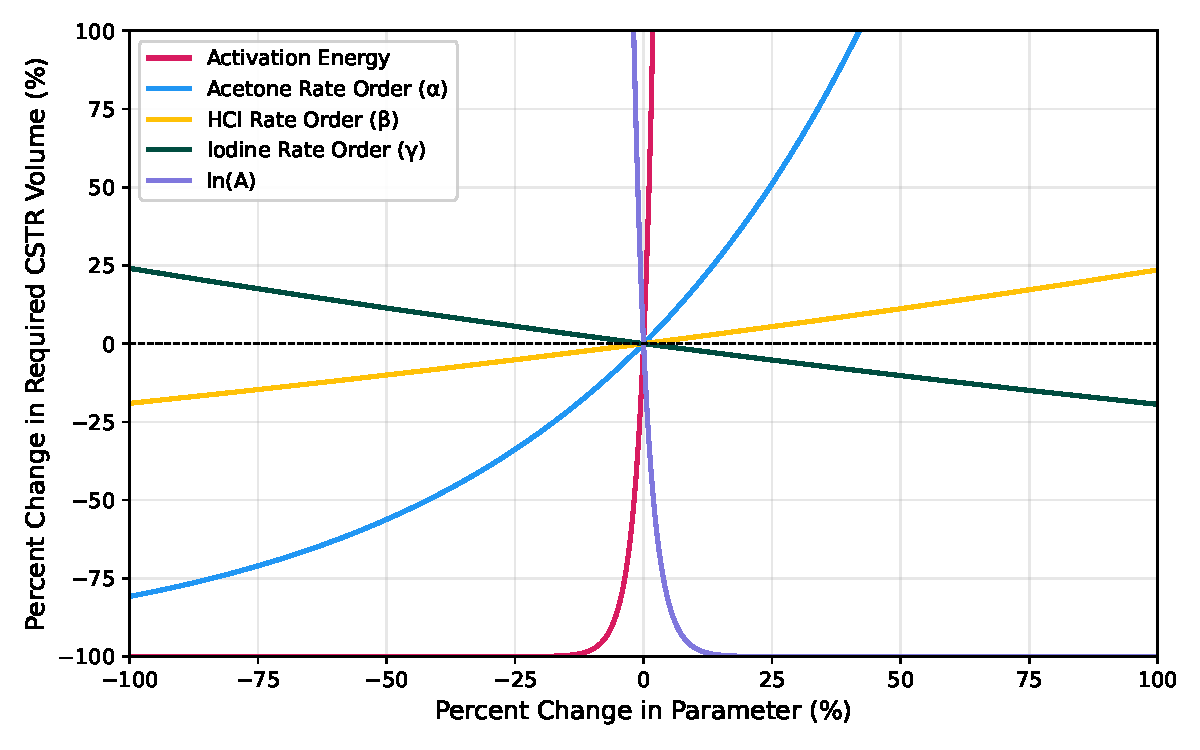
\includegraphics[width=0.9\linewidth]{figures/spider_sensitivity.pdf}
    \caption{Spider plot showing sensitivity of each parameter.}
    \label{fig:spiderplot}
\end{figure}

In \cref{fig:spiderplot}, each kinetic parameter was varied from 0 to 100\% above its nominal value while holding all others fixed. The Arrhenius parameters Ea and $\ln(A)$ produce the steepest response in required reactor volume, reflecting their appearance in the exponential terms of the rate expression. At 80\% conversion, a change in $\alpha$ is more sensitive than that of $\beta$ despite having nearly the same dependence in the rate equation. Acetone has been mostly consumed (down to 0.2 M) at this point while the hydronium concentration is close to 1 (0.801 M) where $\ln(C_{\mathrm{H_3O^+}})$ nearly vanishes.



\begin{table}[H]
    \caption{Sensitivity of derived rate law parameters}
    \centering
    \begin{tabular}{l|ccc}
    \toprule
    Parameter & Sensitivity & Relative Sensitivity \\
    \midrule
    $E_a$ & $\pm 180.7 \ \mathrm{L}$ & $\pm 65.9\%$ \\
    $\ln(A)$ & $\pm 212.6 \ \mathrm{L}$ & $\pm 77.5\%$ \\
    $\alpha$ & $\pm 5.3 \ \mathrm{L}$ & $\pm 1.9\%$ \\
    $\beta$ & $\pm 0.8 \ \mathrm{L}$ & $\pm 0.3\%$ \\
    $\gamma$ & $\pm 5.7 \ \mathrm{L}$ & $\pm 2.1\%$ \\
    \bottomrule
    \end{tabular}
    \label{tab:sensitivity}
\end{table}


The sensitivity analysis reveals that uncertainty in the Arrhenius parameters $E_a$ and $\ln(A)$ dominates the total uncertainty, contributing $\pm 66\%$ and $\pm 78\%$ relative uncertainty to $V$, respectively. Since both terms appear inside an exponential, this was fully anticipated. Small errors in $E_a$ and $\ln(A)$ are amplified nonlinearly into large errors in the rate constant $k$, and consequently in the reactor volume. In contrast to the Arrhenius parameters, the reaction orders $\alpha$, $\beta$, and $\gamma$ each contribute less than 2\% relative uncertainty, making them minor sources of error. 

A subtle result emerges when taking a closer look at the sensitivity to $\beta$ (HCl order, $\pm 0.3\%$) versus $\gamma$ (Iodine order, $\pm 2.1\%$), despite $\gamma$ being nearly zeroth order while $\beta$ is nearly first order. This paradox is resolved by recognizing that the sensitivity of the rate to an exponent parameter scales with the logarithm of the corresponding concentration. At 80\% conversion, $C_I = 0.2 \ \mathrm{M}$ giving $\ln(C_I) = -1.61$, while $C_H = 0.801 \ \mathrm{M}$ giving $\ln(C_H) = -0.22$. The iodine concentration is nearly depleted at this point in the reaction, amplifying the influence of $\gamma$ on the rate. Meanwhile, the hydronium concentration generated by reaction offsets the low initial HCl concentration, keeping $C_{\mathrm{H_3O^+}}$ close to 1 M and minimizing the influence of $\beta$. The sensitivity ranking is specific to the operating conditions and would shift depending on the desired conversion.

Given that $E_a$ and $\ln(A)$ are the dominant uncertainty sources, the most efficient experiments for improving volume prediction would be additional rate measurements across a wider temperature range. The current Arrhenius parameters were regressed from data around 303 K, and extrapolation to 353 K amplifies the uncertainty. Running initial-rate experiments at several temperatures between 303--353 K would constrain $E_a$ and $\ln(A)$ in the regime relevant to the reactor design, and would be more impactful than collecting additional concentration dependence to refine $\alpha$, $\beta$, or $\gamma$.








\subsection{Conclusions and Recommendations}

The acid-catalyzed iodination of acetone was found to follow a rate law that is approximately first order in both acetone and HCl and zeroth order in iodine, consistent with the pseudo equilibrium mechanism \autocite{dongxia}. Nonlinear regression yielded the most precise parameter estimates ($\alpha = 1.026 \pm 0.063$, $\beta = 0.954 \pm 0.068$, $\gamma = -0.134 \pm 0.067$, 95\% CI), and an activation energy of $E_a = (114.4 \pm 5.6) \ \mathrm{kJ \, mol^{-1}}$ and $\ln(A) = (36.0 \pm 2.2)$ (standard errors) were determined from the Arrhenius plot. These parameters were used to model autocatalytic behavior in a BSTR and to size a CSTR for iodoacetone production at 353 K.

The nominal CSTR volume required to achieve 80\% acetone conversion was estimated to be approximately 274 L. However, the 90\% confidence interval derived from a Monte Carlo simulation spans 58--1,290 L, driven mainly by uncertainty in $E_a$ and $\ln(A)$. For the conservative pilot factory design, the upper confidence bound was suggested as the design volume. To most efficiently reduce this uncertainty, additional kinetic experiments should be performed across a wider temperature range between 303--353 K, as this would constrain the Arrhenius parameters in the relevant regime. Further refinement of the reaction orders would show little improvement to the volume prediction at the studied conditions.

\section{Fundamentals of Pressure Measurement}
The second component of the lab introduced the operation of a pressure measurement system. 
Pressure measurement is critical in chemical process industries, and engineers routinely 
work with a range of sensing technologies such as Bourdon gauges, pressure transducers, 
and differential pressure gauges. Each device is suited to different operating ranges and 
process requirements. This exercise provided hands-on exposure to these instruments as 
well as other supplementary components such as mass flow controllers, rotameters, and 
control valves.

\subsection{Objectives}
The secondary objective was to identify and characterize the components of a pneumatic 
pressure rack, including pressure gauges, transducers, flow controllers, and control valves.

\subsection{Safety}
Pressure was gradually introduced to the pressure rack to prevent system damage, with the 
pressurization rate maintained below the pressure relief valve rating of all lines. The 
system was depressurized by slowly opening the ball valves to release air, ensuring that 
pressure readings did not exceed 60 psi.

\subsection{Background}

The pressure rack system consists of four lines: one main line at the top and three 
additional lines below it.
\\[5mm]
\textbf{Main Line}

\begin{figure}
    \centering
    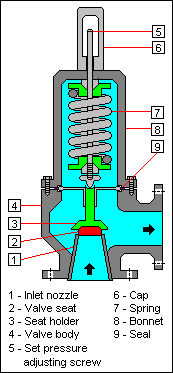
\includegraphics[width=0.2\linewidth]{figures/Pressure_Relief_Valve.png}
    \caption{Pressure relief diagram. \autocite{wikipedia_reliefvalve}}
    \label{fig:pressurereliefdiagram}
\end{figure}

The main line begins with a lockout system, which isolates the pressure source from the 
rest of the system to prevent accidental startup during maintenance. Lockout systems 
typically require multiple locks, and the system cannot be activated until all locks are 
removed.

Downstream of the lockout is a filter, which removes impurities such as water and debris 
from the air supply. When air is compressed, water vapor present in the ambient air is 
concentrated and can condense into liquid water within the system. This moisture can cause 
corrosion, degrade seals, and damage sensitive components such as valves and flow meters. 
The filter serves as the primary protection against water entering the system, reducing 
wear and erosion on system components, extending their service life and preventing failures 
such as pipe bursts or pinhole leaks.

The pressure regulator controls the pressure supplied to the rest of the system. It is 
used to incrementally adjust pressure across multiple measurements and to protect 
downstream components from hazardous pressure levels. Improper handling of this component 
could result in a system rupture.

The lubricator, positioned after the regulator, introduces small amounts of aerosolized 
oil into the airstream to reduce friction and wear on valves, gauges, and other moving 
components. The oil also helps form a seal within the system, reducing the likelihood of 
leakage and extending component lifespan.

The pressure relief valve is set to a maximum allowable pressure. When system pressure 
exceeds this threshold, the valve cap opens to release excess pressure, preventing critical 
pressure buildup that could rupture the system. The relief valve should be set to protect 
the component with the lowest pressure rating in the system. If the relief valve were set 
higher, pressure could rise to a level that exceeds the failure threshold of that component 
before the valve actuates, resulting in a rupture or catastrophic failure. The relief valve 
connects to the receiving vessel below and a ball valve to the right.

A ball valve controls flow by rotating a sphere with a through-hole along its axis. 
Aligning the hole with the flow path opens the valve; misaligning it cuts off flow. The 
state of a ball valve can be confirmed by visual inspection without instrumentation: when 
the handle is parallel to the pipe, the valve is open; when the handle is perpendicular 
to the pipe, the valve is closed. This straightforward design is widely used in industrial 
pressure systems.

\begin{figure}[H]
    \centering
    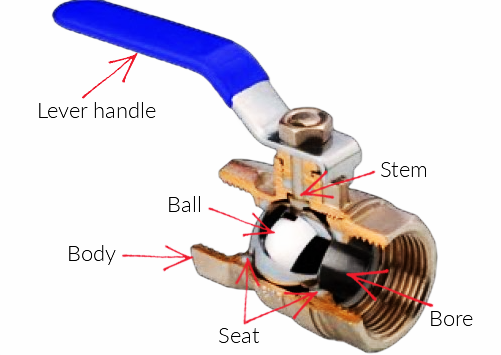
\includegraphics[width=0.5\linewidth]{figures/Ball_Valve.png}
    \caption{Ball valve diagram. \autocite{hosemaster_ballvalve}}
    \label{fig:ballvalvediagram}
\end{figure}

The receiving vessel, located directly below the pressure relief valve, stores compressed 
gas to act as a buffer, maintaining system pressure and reducing the cycle rate of the 
compressor.

Pressure in the main line is measured using a C-type Bourdon gauge, which operates on the 
principle that increased pressure causes a sealed, C-shaped tube to straighten and expand. 
This deflection is translated into a pressure reading displayed on the gauge face. The 
Bourdon gauge measures gauge pressure, which is defined relative to ambient atmospheric 
pressure rather than a perfect vacuum. Gauge pressure and absolute pressure are related by:

\begin{equation}
    P_{\text{gauge}} = P_{\text{absolute}} - P_{\text{atmospheric}}
\end{equation}

Two Bourdon gauges are present on the first line with different full-scale ranges. The 
gauge with the smaller range was used for this experiment, as the larger gauge was observed 
to read approximately half the pressure indicated by all other gauges in the system, 
suggesting it was either miscalibrated or operating well outside its accurate range. A 
gauge whose full-scale range closely brackets the operating pressures of the experiment 
produces readings with greater resolution and lower relative error than one with a much 
larger range, as an oversized scale compresses the relevant portion of the display and 
increases measurement uncertainty. Bourdon gauges remain widely used in industrial 
pressure systems. A digital gauge is also present on the first line, using internal 
components such as a strain gauge or piezoresistive sensor to measure and display pressure 
electronically.

\begin{figure}[H]
    \centering
    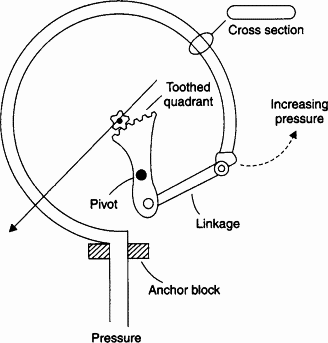
\includegraphics[width=0.3\linewidth]{figures/Bourdon_Gauge.png}
    \caption{Bourdon gauge diagram. \autocite{sciencedirect_bourdon}}
    \label{fig:bourdongaugediagram}
\end{figure}

\noindent
\textbf{Second Line}

The second line is toggled from the main line via a ball valve. It contains a mass flow 
controller (MFC), which measures and regulates gas flow using a proportional control valve 
and a closed-loop control system. The user provides an input signal, which the MFC 
compares against its internal mass flow sensor to adjust the valve accordingly. Flow rate 
is expressed as a percentage of the MFC's calibrated full-scale value.

\begin{figure}[H]
    \centering
    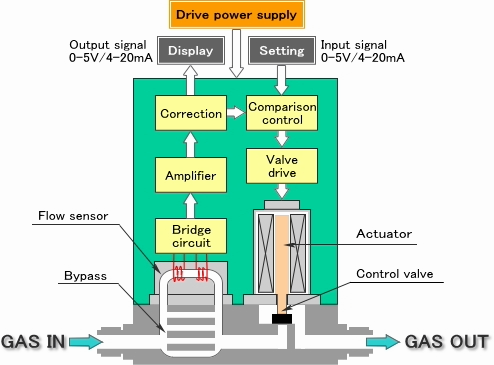
\includegraphics[scale=0.75]{figures/MFC.png}
    \caption{Mass flow controller diagram. \autocite{fcon_mfc}}
    \label{fig:massflowcontrollerdiagram}
\end{figure}

A rotameter is attached downstream of the MFC and serves as its calibration reference. 
The rotameter is a variable-area flow meter that operates by passing air through a tapered 
tube, raising a float proportionally to the flow rate. Unlike the MFC, the rotameter 
requires no power and is simple in construction.

\begin{figure}[H]
    \centering
    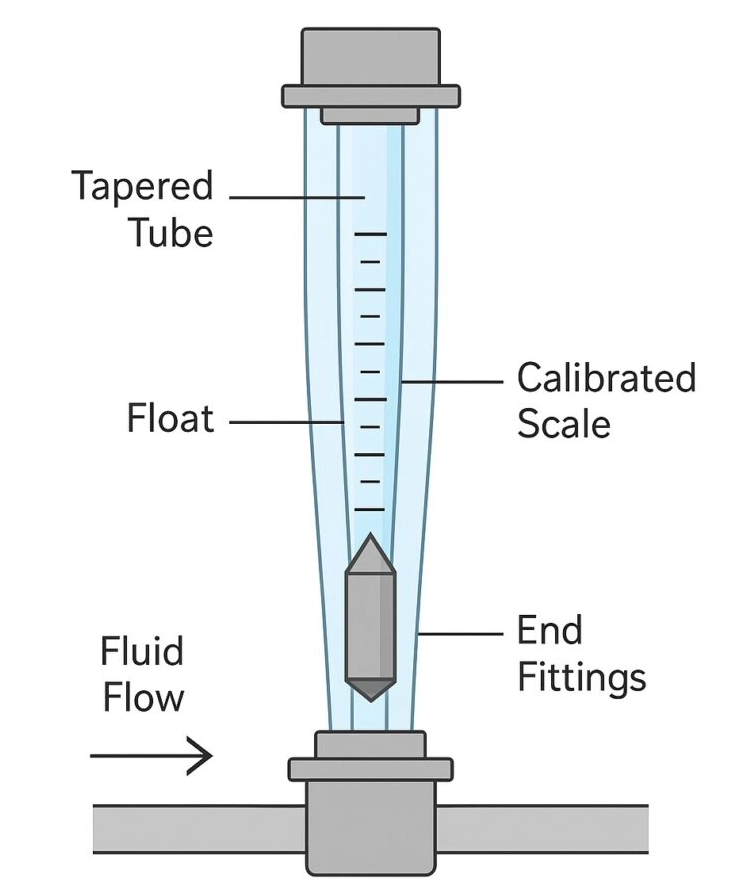
\includegraphics[scale=0.3]{figures/Rotameter.png}
    \caption{Rotameter diagram. \autocite{valuemax_rotameter}}
    \label{fig:rotameterdiagram}
\end{figure}

\noindent
\textbf{Third Line}

The third line contains a pressure transducer, which measures pressure and converts it to 
an electrical signal read and displayed by a connected computer. This type of sensor is 
common across industrial, automation, and off-road equipment applications. A Bourdon gauge 
is also present on this line, operating as described above.
\\[5mm]
\textbf{Fourth Line}

The fourth line includes a pressure regulator fixed at 15 psi, connected to an 
electro-pneumatic transducer (I/P transducer). Unlike the regulator on the main line, 
this regulator does not actively set system pressure. It is still controlled by 
the primary regulator, and this one follows accordingly. The I/P transducer converts a 
DC electrical current into a proportional pneumatic pressure signal, displayed on an 
analog dial. This pneumatic signal is used to actuate a control valve downstream, forming 
a complete electro-pneumatic control loop. As the input current to the I/P transducer is 
varied, the output pressure signal changes proportionally, which in turn adjusts the 
position of the control valve and regulates flow through the line. This arrangement is 
common in industrial process control, as it allows an electronic control system to 
manipulate pneumatic field devices without requiring direct mechanical intervention, 
enabling precise and automated flow regulation.

\subsection{Pneumatic Controls in Industrial Settings}

Pneumatic control systems are widely used in industry because they are reliable, 
cost-effective, and inherently safe in hazardous environments where electrical systems 
may pose ignition risks \autocite{dindorf_review_2025}. Compressed air is readily 
available in most industrial facilities and requires no return line, simplifying system 
design. Pneumatic actuators can generate large forces at relatively low cost, making them 
well suited for controlling valves, clamps, and other mechanical systems at scale. 
Additionally, pneumatic systems are tolerant of temperature extremes and present no 
electrical shock hazard, making them preferable in environments such as chemical plants, 
mining operations, and food processing facilities.

The U-tube manometer and Magnehelic gauge are additional pressure measurement devices 
commonly encountered in engineering practice; however, as these instruments were not 
present in the laboratory, they are not discussed further in this report.

\subsection{Methods}

The lockout system, filter, regulator, lubricator, and pressure relief valve were 
identified at the inlet of the system. The electronic components were then powered on, 
the lockout was disengaged, and the ball valves were opened slowly to establish airflow.

At the first line, the Bourdon and digital pressure gauges were identified and their 
pressure readings were recorded. At the second line, the mass flow controller and 
rotameter were identified and their readings recorded. At the third line, the Bourdon 
gauge and pressure transducer were identified and their pressures recorded. At the fourth 
line, the pressure regulator was set to 15 psi, and the I/P transducer and pneumatic valve 
were examined and their pressures recorded.

The hand regulator was then used to observe the effect of the three-way valve position on 
system pressure. With the three-way valve closed, the vessel was observed to decompress; 
with it open, system pressure was maintained. To generate the MFC calibration curve, the 
rotameter was set to flow rates of 1000, 800, 600, 400, and 200 CCM, and the corresponding 
MFC readings were recorded at each point. These values were then plotted to establish the 
relationship between the two instruments. To generate the pressure transducer calibration 
curve, system pressure was adjusted so that the Bourdon gauge read values of 40, 35, 30, 
25, and 20 psi. The corresponding transducer output was recorded at each setpoint, and 
the two datasets were plotted against each other to produce the calibration curve.

\subsection{Results}

The calibration curves for the pressure transducer and mass flow controller are presented in Figures~\ref{fig:bourdon} and~\ref{fig:rotameter}, respectively.

\begin{figure}[H]
    \centering
    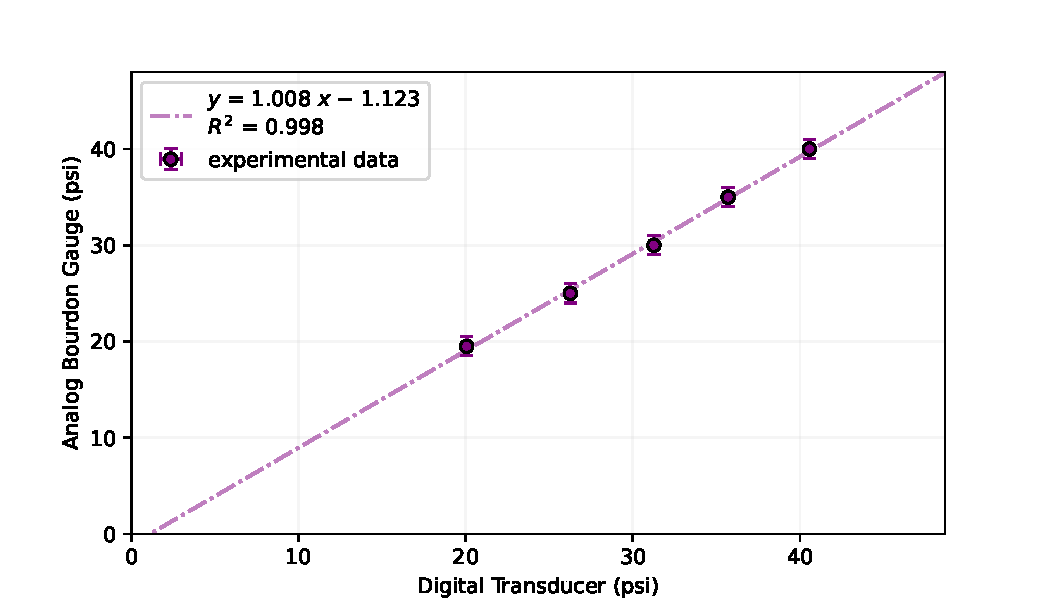
\includegraphics[width=0.8\linewidth]{figures/bourdon.pdf}
    \caption{Calibration curve for the pressure transducer. Analog Bourdon gauge pressure is plotted against digital transducer pressure. A linear fit yields $P_{\mathrm{Bourdon}} = 1.008\, P_{\mathrm{transducer}} - 1.123$ with $R^2 = 0.998$, indicating strong agreement between the two instruments.}
    \label{fig:bourdon}
\end{figure}

\begin{figure}[H]
    \centering
    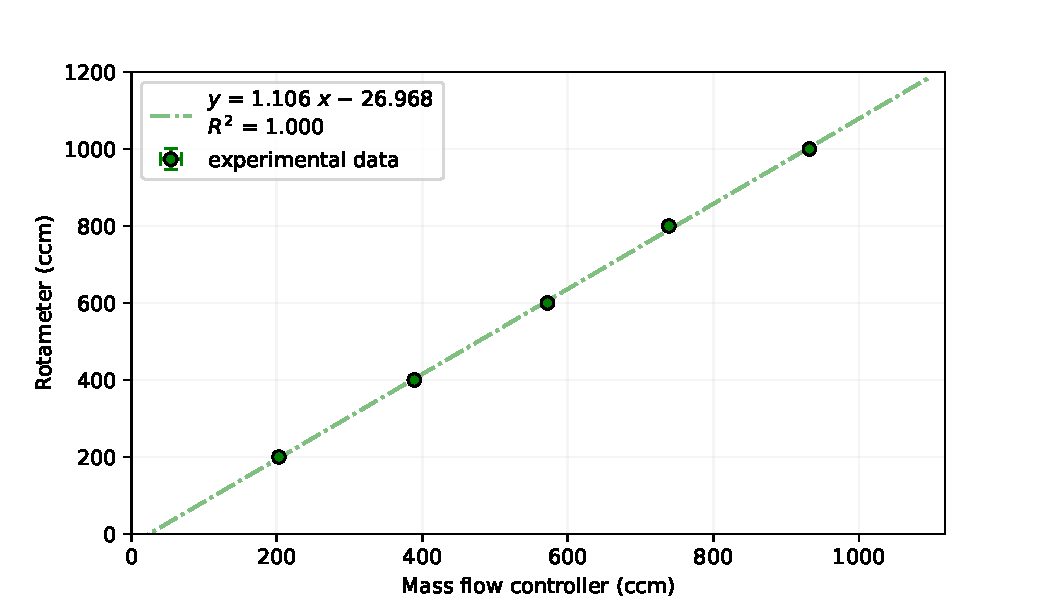
\includegraphics[width=0.8\linewidth]{figures/rotameter.pdf}
    \caption{Calibration curve for the mass flow controller. Rotameter flow rate is plotted against MFC flow rate. A linear fit yields $\dot{V}_{\mathrm{rotameter}} = 1.106\, \dot{V}_{\mathrm{MFC}} - 26.968$ with $R^2 = 1.000$, indicating an excellent linear relationship across the measured range.}
    \label{fig:rotameter}
\end{figure}

 The transducer calibration yielded a slope of approximately unity ($m = 1.008$) with a small offset ($b = -1.123$ psi) and $R^2 = 0.998$, indicating that the digital transducer and analog Bourdon gauge are in close agreement across the measured range. The small offset suggests a minor systematic difference between the two instruments, which may be attributed to Bourdon gauge resolution limitations or a slight zero-offset in the transducer. Using the linear fit, pressure may be determined from the transducer signal as:

\begin{equation}
    P_{\text{Bourdon}} = 1.008\, P_{\text{transducer}} - 1.123
\end{equation}

The MFC calibration yielded a slope of $m = 1.106$ with an offset of $b = -26.968$ ccm and $R^2 = 1.000$, indicating an essentially perfect linear relationship between the MFC and rotameter readings. The slope greater than unity suggests the MFC consistently reads slightly lower than the rotameter, which may reflect a calibration offset in the MFC relative to the reference rotameter. Using the linear fit, flow rate may be determined from the MFC signal as:

\begin{equation}
    \dot{V}_{\text{rotameter}} = 1.106\, \dot{V}_{\text{MFC}} - 26.968
\end{equation}

Calibration of these instruments is important because both the pressure transducer and MFC report electronic signals that must be related to physical quantities through a known reference. Without calibration, systematic offsets between instruments would introduce error into any measurements or process control decisions that depend on them. The strong linearity observed in both calibration curves confirms that both instruments 
are functioning correctly within the measured range and that their outputs can be reliably converted using the derived equations.

\printbibliography

\appendix
\crefalias{section}{appendix}
\crefalias{subsection}{appendix}
\crefalias{subsubsection}{appendix}
\section{Appendices}
\subsection{SDS Information} % This will be Appendix A
\label{app:SDS}

\begin{tabular}{p{0.18\linewidth}p{0.3\linewidth}p{0.5\linewidth}}
\toprule
Chemical & Hazards & Treatments \\
\midrule
Acetone & Flammable in both its liquid and vapor forms, may cause irritation of respiratory tract, vapors may cause drowsiness, and repeated exposure may cause skin dryness. & Rinse eyes immediately upon contact, wash skin immediately upon contact, move to fresh air if inhaled, and obtain medical attention if ingested. \\ \\
Hydrochloric acid & Corrosive to metals, may cause skin corrosion/irritation, eye damage/irritation, and respiratory system toxicity. & Rinse eyes immediately upon contact, wash skin immediately upon contact, call Poison Center Control if ingested, and move to fresh air if inhaled. \\ \\
Hydrogen iodide & Corrosive to the respiratory system, eyes, and skin, harmful/toxic if inhaled, and causes burns. & Rinse eyes immediately upon contact, wash skin immediately upon contact, move to fresh air if inhaled, wash out mouth with water and seek medical attention if ingested. \\ \\
Iodine water & Irritating to skin and body tissues. & Rinse eyes immediately upon contact, wash skin immediately upon contact, move to fresh air if inhaled, and rinse out mouth with water or milk, induce vomiting, and seek medical attention if ingested. \\
\bottomrule
\end{tabular}
\subsubsection*{SDS references}
\begin{enumerate}
    \item Fisher Scientific. Acetone Material Safety Data Sheet. 2009. \url{https://udel.instructure.com/courses/1903743/files/folder/KIN%20Resources/2025/1.%20MSDS?preview=156346371}

    \item Fisher Scientific. Hydrochloric Acid Material Safety Data Sheet. 2009. \url{https://udel.instructure.com/courses/1903743/files/folder/KIN%20Resources/2025/1.%20MSDS?preview=156346373}

    \item ThermoFisher Scientific. Hydrochloric Acid Safety Data Sheet. 2009. \url{https://www.fishersci.com/store/msds?partNumber=A481212&productDescription=HYDROCHLORIC+ACID+NF%2FFCC+21%2F2L&vendorId=VN00033897&countryCode=US&language=en}

    \item Fisher Scientific. Hydrogen Iodide Material Safety Data Sheet. 2009. \url{https://udel.instructure.com/courses/1903743/files/folder/KIN%20Resources/2025/1.%20MSDS?preview=156346372}

    \item Flinn Scientific Inc. Iodine Water Material Safety Data Sheet. 2002. \url{https://udel.instructure.com/courses/1903743/files/folder/KIN%20Resources/2025/1.%20MSDS?preview=156346380}
\end{enumerate}



\subsection{Data Processing}
\label{app:processing}

Each individual signal was processed through the following pipeline
\begin{enumerate}
    \item The absorbance values in the signal were converted to concentration values using the calibration curve for the UV-vis spectrophotometer used to collect the signal.
    \item From there, outliers were removed from the signal using random sample consensus RANSAC \autocite{RANSAC} as the outliers are “gross” meaning the significant outliers are strictly greater than the mean and not normally distributed about the mean.
    \item A loss function of absolute error was used and considered points with a residual greater than 0.00001 M as outliers.
    \item A line was then fit to the concentration data and the slope saved as the reaction rate. 
\end{enumerate}
To obtain temperature for each reaction, the start time of the reaction was noted. For a reaction with n absorbance measurements, n temperature measurements were considered after the noted start time when calculating the average and standard deviation. An illustration of outlier removal with RANSAC is shared below.

\begin{figure}[H]
    \centering
    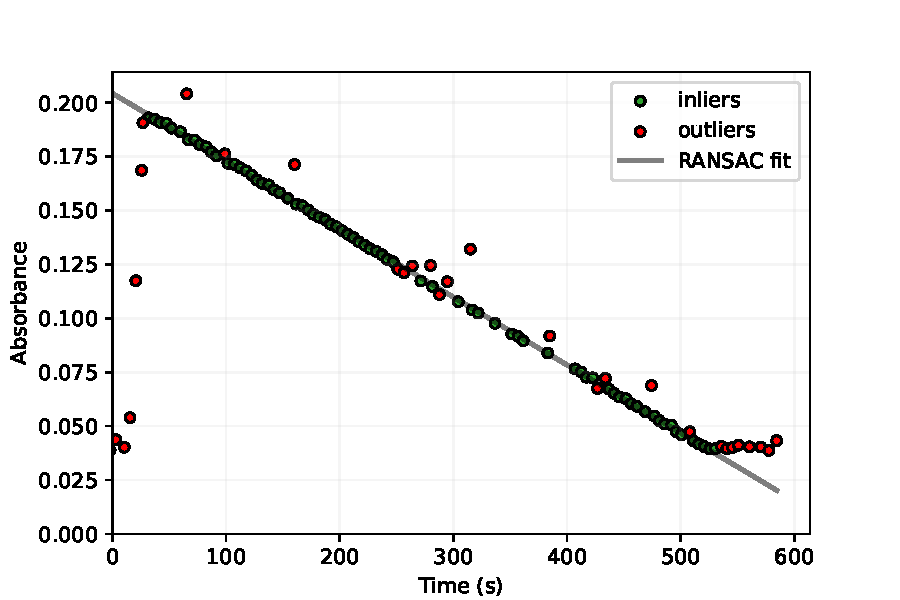
\includegraphics[width=0.8\linewidth]{figures/RANSAC.pdf}
    \caption{Illustrative RANSAC outlier detection. The red points have been identified as outliers and it should be noted that the outliers are almost strictly above the mean as opposed to being distributed normally around the mean.}
    \label{fig:ransac}
\end{figure}



\subsection{Reaction Order Data}
\label{app:orderData}
This data is additionally available for download on Github \url{https://github.com/kylecapybara/cheg345kin}.

\begin{table}[H]
\centering
\caption{Experimental data for iodination of acetone under varying conditions.}

\begin{subtable}{\textwidth}
\centering
\caption{Collected data for determining reaction order with respect to hydrochloric acid.}
\begin{tabular}{rrrrr}
\toprule
Temperature (ºC) & [HCl] (M) & [I$_2$] (M) & [Acetone] (M) & Rate (M/s) \\
\midrule
2.956e+01 & 2.411e-02 & 2.130e-03 & 1.990e+00 & 4.700e-06 \\
2.941e+01 & 1.134e-02 & 2.290e-03 & 1.980e+00 & 2.170e-06 \\
2.936e+01 & 4.082e-02 & 2.000e-03 & 1.970e+00 & 7.570e-06 \\
\bottomrule
\end{tabular}
\end{subtable}

\vspace{0.75em}

\begin{subtable}{\textwidth}
\centering
\caption{Collected data for determining reaction order with respect to iodine}
\begin{tabular}{rrrrr}
\toprule
Temperature (ºC) & [HCl] (M) & [I$_2$] (M) & [Acetone] (M) & Rate (M/s) \\
\midrule
2.956e+01 & 2.411e-02 & 2.130e-03 & 1.990e+00 & 4.700e-06 \\
2.927e+01 & 2.054e-02 & 4.180e-03 & 1.950e+00 & 3.570e-06 \\
2.956e+01 & 2.094e-02 & 1.030e-03 & 1.990e+00 & 4.460e-06 \\
\bottomrule
\end{tabular}
\end{subtable}

\vspace{0.75em}

\begin{subtable}{\textwidth}
\centering
\caption{Collected data for determining reaction order with respect to acetone}
\begin{tabular}{rrrrr}
\toprule
Temperature (ºC) & [HCl] (M) & [I$_2$] (M) & [Acetone] (M) & Rate (M/s) \\
\midrule
2.956e+01 & 2.411e-02 & 2.130e-03 & 1.990e+00 & 4.700e-06 \\
2.927e+01 & 2.009e-02 & 3.010e-03 & 4.660e-01 & 7.330e-07 \\
2.974e+01 & 2.069e-02 & 2.150e-03 & 4.030e+00 & 8.210e-06 \\
\bottomrule
\end{tabular}
\end{subtable}

\end{table}




\subsection{Collected Signals}
\label{app:signals}

\cref{fig:collectedsignals} shares all of collected signals with outliers removed and the peak absorbance set to a time of zero seconds. 

\begin{figure}[H]
    \centering
    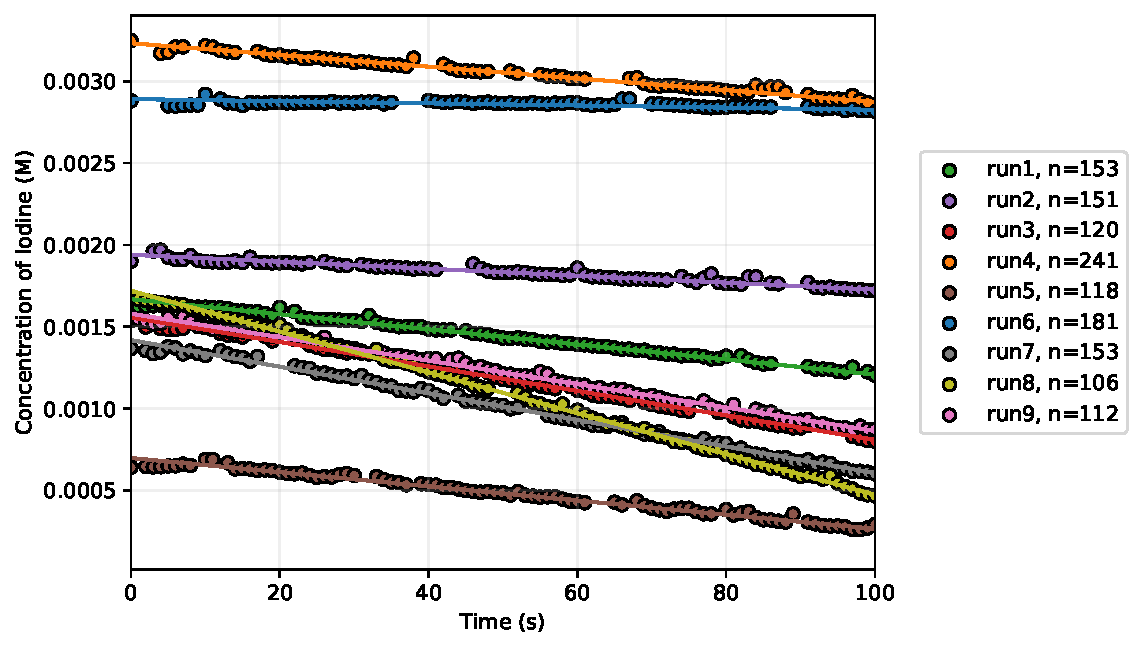
\includegraphics[width=0.75\linewidth]{figures/collecteddata.pdf}
    \caption{Collected signals with outliers removed and linear fits.}
    \label{fig:collectedsignals}
\end{figure}

These collected signals were converted from absorbance to concentrating using the following calibration curves as provided by the instructional team. The provided calibration curves are shared below in \cref{fig:calibrationcurve}.

\begin{figure}[H]
    \centering
    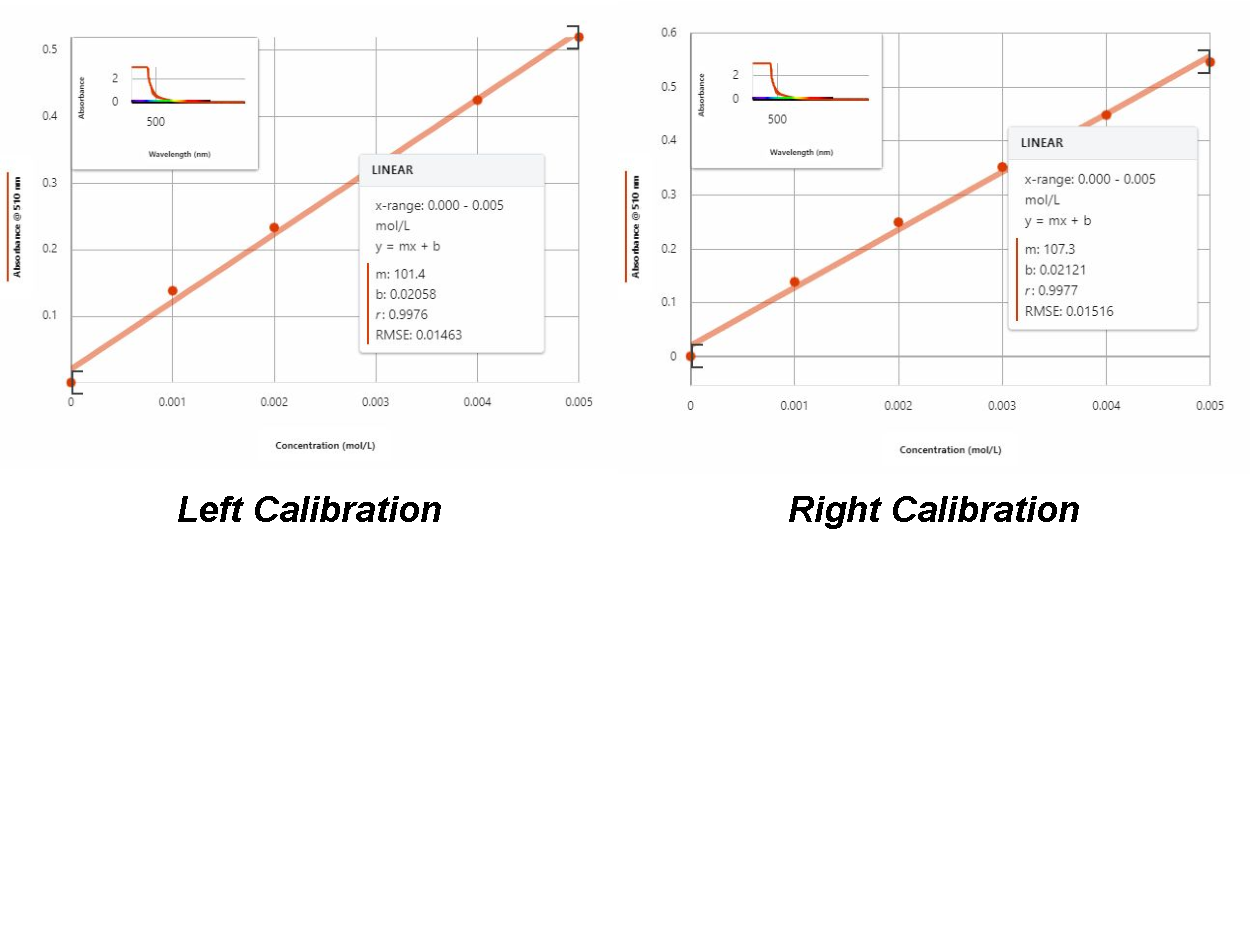
\includegraphics[width=0.9\linewidth]{figures/calibration.pdf}
    \caption{Calibration curves relating iodine concentration to absorbance.}
    \label{fig:calibrationcurve}
\end{figure}


\subsection{Propagation of Uncertainty}
\label{app:errorProp}

Rearranging the linearized rate law arrives at equation \cref{eq:lnk},

\begin{equation}
    \ln(k) = \ln(\mathrm{Rate}) - \alpha \ln([\mathrm{Ac}]) - \beta \ln([\mathrm{H_3O^+}]) - \gamma \ln([\mathrm{I_2}])
    \label{eq:lnk}
\end{equation}

Treating the uncertainties in concentration as negligible, the uncertainty in $\ln(k)$ arises from the uncertainties in the fitted exponents $\alpha$, $\beta$, $\gamma$, and in the measured rate. Applying standard propagation of uncertainty to \cref{eq:lnk}:

\begin{equation}
    \delta \ {\ln(k)} = \sqrt{
        \left(\frac{\partial \ln(k)}{\partial \ln(\mathrm{Rate})}\,\delta \ {\ln(\mathrm{Rate})}\right)^2
      + \left(\frac{\partial \ln(k)}{\partial \alpha}\,\delta\alpha\right)^2
      + \left(\frac{\partial \ln(k)}{\partial \beta}\,\delta\beta\right)^2
      + \left(\frac{\partial \ln(k)}{\partial \gamma}\,\delta\gamma\right)^2
    }
\end{equation}
Evaluating each partial derivative from \cref{eq:lnk},

\begin{align*}
    \frac{\partial \ln(k)}{\partial \ln(\mathrm{Rate})} &= 1 \\[4pt]
    \frac{\partial \ln(k)}{\partial \alpha} &= -\ln([\mathrm{Ac}]) \\[4pt]
    \frac{\partial \ln(k)}{\partial \beta}  &= -\ln([\mathrm{H_3O^+}]) \\[4pt]
    \frac{\partial \ln(k)}{\partial \gamma} &= -\ln([\mathrm{I_2}])
\end{align*}
Substituting,

\begin{equation}
    \delta \ {\ln(k)} = \sqrt{
        \left(\delta \ {\ln(\mathrm{Rate})}\right)^2
      + \bigl(\ln([\mathrm{Ac}])\,\delta\alpha\bigr)^2
      + \bigl(\ln([\mathrm{H_3O^+}])\,\delta\beta\bigr)^2
      + \bigl(\ln([\mathrm{I_2}])\,\delta\gamma\bigr)^2
    }
    \label{eq:pou_lnk1}
\end{equation}
The uncertainty in $\ln(\mathrm{Rate})$ is obtained by propagating $\delta\mathrm{Rate}$ through the logarithm:
\begin{equation*}
    \delta\ln(\mathrm{Rate}) = \left|\frac{d\ln(\mathrm{Rate})}{d\,\mathrm{Rate}}\right| \delta\mathrm{Rate} = \frac{\delta\mathrm{Rate}}{\mathrm{Rate}}
\end{equation*}
Substituting this result into \cref{eq:pou_lnk1} yields the following (as presented earlier in the body of this report).
\begin{equation}
    \delta \ {\ln(k)} = \sqrt{
        \left( {\frac{\delta\mathrm{Rate}}{\mathrm{Rate}}}\right)^2
      + \bigl(\ln([\mathrm{Ac}])\,\delta\alpha\bigr)^2
      + \bigl(\ln([\mathrm{H_3O^+}])\,\delta\beta\bigr)^2
      + \bigl(\ln([\mathrm{I_2}])\,\delta\gamma\bigr)^2
    }
    \label{eq:pou_lnk2}
\end{equation}
It should be noted that a formula derived not neglecting the contributions from the error in the concentrations was tested and produced error bars indistinguishable from the result neglecting the error in concentrations.

\subsection{Statistical Tests}
\label{app:tests}

All tests were two-tailed $t$-tests implemented using \texttt{scipy.stats.t}.

\subsubsection*{Hypothesis Framework}

For each parameter $\theta$ with estimated value $\hat{\theta}$ and standard error $s_{\hat{\theta}}$,
the null hypothesis is that the parameter equals the theoretical or literature value $\theta_0$:
\begin{equation}
    H_0: \theta = \theta_0 \qquad H_a: \theta \neq \theta_0
\end{equation}
The t-statistic is then
\begin{equation}
    t = \frac{\hat{\theta} - \theta_0}{s_{\hat{\theta}}}
\end{equation}
where the standard error is estimated from the sample standard deviation, $\sigma$, of the estimated parameter values across the $N$ repeated measurements,
\begin{equation}
    s_{\hat{\theta}} = \frac{\sigma}{\sqrt{N}}
\end{equation}
P-values were computed from the two-tailed cumulative distribution function of the $t$-distribution at $\nu = N - n$ degrees of freedom where $N$ is the number of collected data points and $n$ is the number of fit model parameters.

\subsubsection*{Reaction Orders}

Reaction orders were tested against the theoretical values predicted by the pseudo-equilibrium mechanism: $\alpha_0 = 1$, $\beta_0 = 1$, $\gamma_0 = 0$. For each species, three repeated measurements were collected at varying concentration of that species while holding all others fixed, giving $N = 3$ and $\nu = 1$ degrees of freedom. 

\subsubsection*{Activation Energy}

The experimentally determined activation energy was compared against the literature value reported by Albery and Robinson \cite{albery_measurement_1969} of $E_{a,\mathrm{lit}} = 86.60\ \mathrm{kJ\ mol^{-1}}$. The literature value is treated as a known population parameter. Rate constants were computed at each of the three experimental temperatures, giving $N = 3$ and $\nu = 1$ degrees of freedom. The standard error of $\hat{E}_a$ is therefore \cref{eq:seEa} where $\sigma_m$ is the standard error of the slope of the regression line which comes from the square root of the diagonal entries of the covariance matrix.
\begin{equation}
    s_{\hat{E}_a} = - R \,\cdot \sigma_m \label{eq:seEa}
\end{equation}
The test statistic is then,
\begin{equation}
    t = \frac{\hat{E}_a - E_{a,\mathrm{lit}}}{s_{\hat{E}_a}}
    = \frac{(111{,}200 - 86{,}600)\ \mathrm{J\ mol^{-1}}}{s_{\hat{E}_a}}.
\end{equation}
This yields $t = 4.98$ at $\nu = 1$, giving $p = 0.126$, indicating  statistical agreement with the literature consensus. 

\subsection{Plotting Confidence Intervals}
\label{app:plotCI}
To generate 95\% confidence interval on plots with linear regression the following equations were used.

\[
x_i=\frac{1}{T_i},\qquad y_i=\ln(k_i),\qquad \hat y(x)=\hat\beta_0+\hat\beta_1 x
\]
\[
s=\sqrt{\frac{\sum_{i=1}^{n}(y_i-\hat y_i)^2}{n-2}},\qquad
S_{xx}=\sum_{i=1}^{n}(x_i-\bar x)^2
\]
From these equations, the 95\% CI upper and lower bounds are given by $\hat{y}_{x_0}$ as shared in \cref{eq:CIlines}.
\begin{equation}
    \hat y(x)\pm t_{0.975,\;n-2}\,s\sqrt{\frac{1}{n}+\frac{(x-\bar x)^2}{S_{xx}}} \label{eq:CIlines}
\end{equation}

\subsection{Pressure Rack Data}
\label{app:pressure}

\begin{table}[H]
    \centering
    \caption{Pressures in First Flow Line}
    \label{tab:firstflowline}
    \begin{tabular}{lccccc}
        \toprule
        & P1 & P2 & P3 & P4 & P5 \\
        \midrule
        Bourdon Gauge (psi)        & 10.0 & 11.0 & 16.5 & 19.0 & 20.0 \\
        Digital Gauge (MPa)        & 0.139 & 0.179 & 0.206 & 0.243 & 0.280 \\
        Other Bourdon Gauge (psi)  & 20.0 & 26.0 & 30.0 & 35.0 & 40.1 \\
        Uncertainty                & 0.1 & 0.1 & 0.1 & 0.1 & 0.1 \\
        \bottomrule
    \end{tabular}
\end{table}

% Requires: \usepackage{booktabs}
\begin{table}[H]
    \centering
    \caption{Pressures in Second Flow Line}
    \label{tab:secondflowline}
    \begin{tabular}{lccccc}
        \toprule
        2nd Line & P1 & P2 & P3 & P4 & P5 \\
        \midrule
        Rotameter     & 1000 & 800 & 600 & 400 & 200 \\
        MFC Set Point & 0.932 & 0.739 & 0.572 & 0.389 & 0.203 \\
        \bottomrule
    \end{tabular}
\end{table}

\begin{table}[H]
    \centering
    \caption{Pressures in Third Flow Line}
    \label{tab:thirdflowline}
    \begin{tabular}{lccccc}
        \toprule
        3rd Line & P1 & P2 & P3 & P4 & P5 \\
        \midrule
        Bourdon Gauge & 19.5 & 25.0 & 30.0 & 35.0 & 40.0 \\
        Transducer    & 20.06 & 26.26 & 31.26 & 35.70 & 40.56 \\
        \bottomrule
    \end{tabular}
\end{table}

\begin{table}[H]
    \centering
    \caption{Pressure \& Electric Signal in Fourth Flow Line}
    \label{tab:fourthflowline}
    \begin{tabular}{ll}
        \toprule
        4th Line                &  \\ \midrule
        Pressure & 15 psi \\
        Pneumatic Valve (psi)   & 16.2 \\
        EM Transducer (V)       & 4.4 \\
        \bottomrule
    \end{tabular}
\end{table}



\subsection{Numerical Simulation of BSTR}
\label{app:bstr}

The python code used to model the autocatalytic behavior in a BSTR is available on Github (\url{https://github.com/kylecapybara/cheg345kin/blob/main/bstr/bstr_UPDATED.ipynb})

\subsection{CSTR Sizing}

The python code used for CSTR sizing and sensitivity analysis is available on Github (\url{https://github.com/kylecapybara/cheg345kin/blob/main/cstrsizing.py})




\end{document}
